\section{Results}
\fxnote{This should be a collaborative section}

\subsection{Domain and grid resolution study}

%%%%%%%%%%%%%%% GRID STUDY: INTEGRAL LENGTH %%%%%%%%%%%%%%%%%%%%%%%%%%%%%%%%%%%
\begin{table}
\caption{\label{tab:GridStudySetup} The setup for the grid resolution study} \centering
\begin{tabular}{ccccc}
  \hline
  Case              & dx [m] & dy [m] & dz [m] \\
  \hline
  Nalu-wind coarse  &  10.0  & 10.0   & 2.5   \\
  Nalu-wind medium  &   5.0  &  5.0   & 2.5   \\
  Nalu-wind fine    &   2.5  &  2.5   & 2.5   \\
  AMR-wind fine     &   2.5  &  2.5   & 2.5   \\
\hline
\end{tabular}
\end{table}

The maximum resolvable frequency on a mesh with grid size $\Delta$ and
average horizontal wind speed $\bar{U}_{horiz}$ can be estimated as
\begin{equation}
  \label{eq:fmax}
  f_{max} = \frac{0.6\bar{U}_{horiz}}{N\Delta}.
\end{equation}
Here, equation \ref{eq:fmax} assumes that the turbulent eddies convect
with a velocity of $0.6\bar{U}_{horiz}$ and $N=8$ is chosen for the
purposes of this study.  Due to the alignment of the flow with the
mesh directions, the grid size $\Delta = \sqrt{2}\cdot \textrm{dx}$.

The wind spectra
\begin{equation}
  \int_0^\infty S_i(f) \textrm{d}f = \sigma_i^2
\end{equation}

%%%%%%%%%%% Grid resolution spectra figure %%%%%%%%%%%%%%%%%%%%%%%%%
% Created in Postprocessing/GridStudy/GridStudy_Spectra.ipynb
\begin{figure}[hbt!]
  \label{fig:GridStudySpectra}
  \centering
  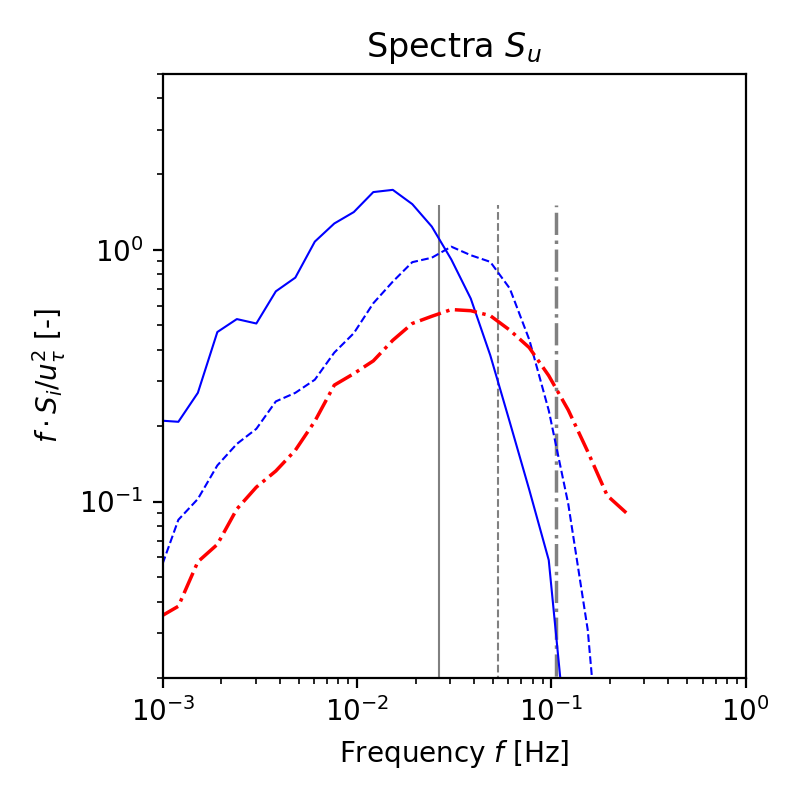
\includegraphics[width=2.0in]{figures/GridStudy_Spectra_Su.png}
  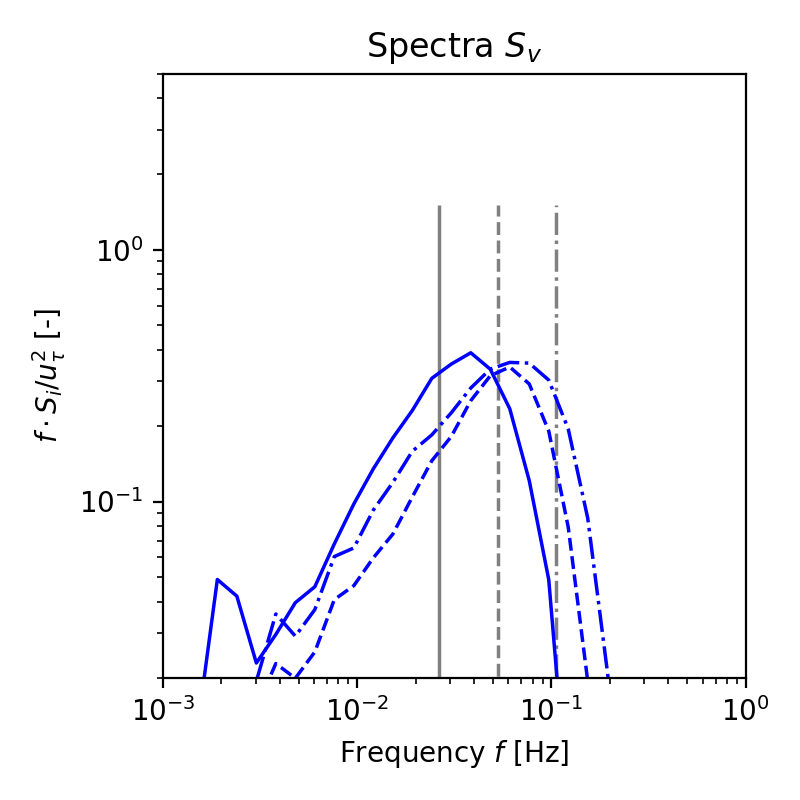
\includegraphics[width=2.0in]{figures/GridStudy_Spectra_Sv.png}
  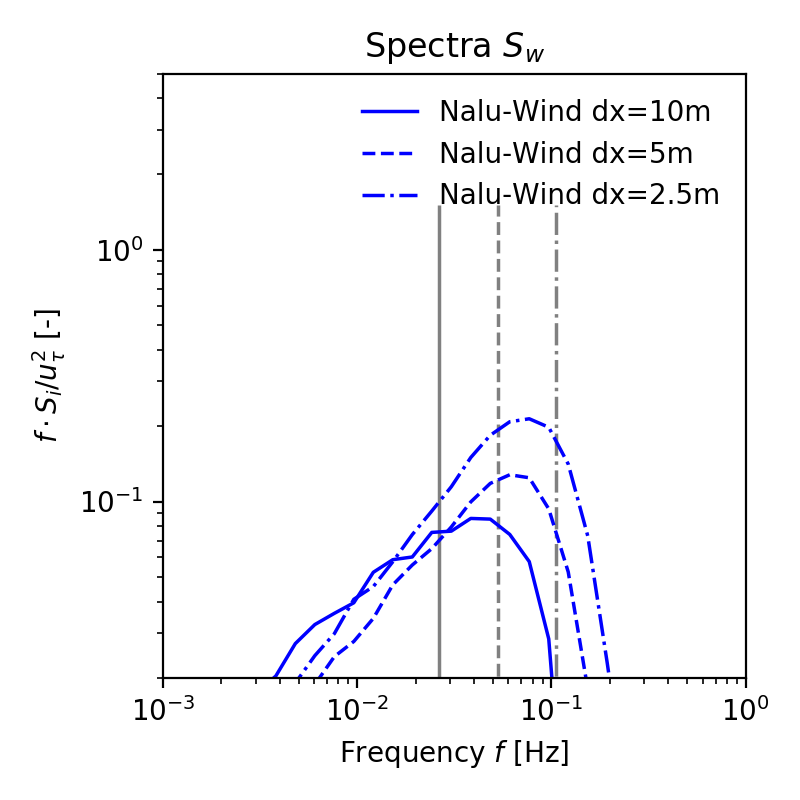
\includegraphics[width=2.0in]{figures/GridStudy_Spectra_Sw.png}
  \caption{Calculation of the wind spectra $S_i$ for LES of stable
    5m/s case with different resolutions.  The gray vertical lines
    correspond to the maximum resolvable frequency according to
    equation (\ref{eq:fmax}). }
\end{figure}
%%%%%%%%%%%%%%%%%%%%%%%%%%%%%%%%%%%%%%%%%%%%%%%%%%%%%%%%%%%%%%%%%%%%

The two-point correlation tensor defined as
\begin{equation}
  \label{eq:Rij}
  R_{ij}({\mathbf x},\boldsymbol{\xi}) = 
  \frac{\overline{ {u'_i(\mathbf{x}, t) u'_j(\mathbf{x}+\boldsymbol{\xi},t)} }}
       { \sqrt{\overline{ u'^2_i }} \sqrt{\overline{ u'^2_j}} }
\end{equation}
where the velocity fluctuations $u'_i$ are defined as 
\begin{equation}
  u'_i(\mathbf{x},t) = u_i(\mathbf{x},t) - \overline{ u_i(\mathbf{x},t) }
\end{equation}

The horizontally averaged correlation coefficient $\langle
R_{ij}(\boldsymbol{\xi})\rangle$ is computed from
$R_{ij}(\mathbf{x},\boldsymbol{\xi})$ by sampling over ...

%%%%%%%%%%% Grid resolution correlation figure %%%%%%%%%%%%%%%%%%%%
% Created in Postprocessing/GridStudy/GridStudy_Rij.ipynb
\begin{figure}[hbt!]
  \label{fig:GridStudyRij}
  \centering
  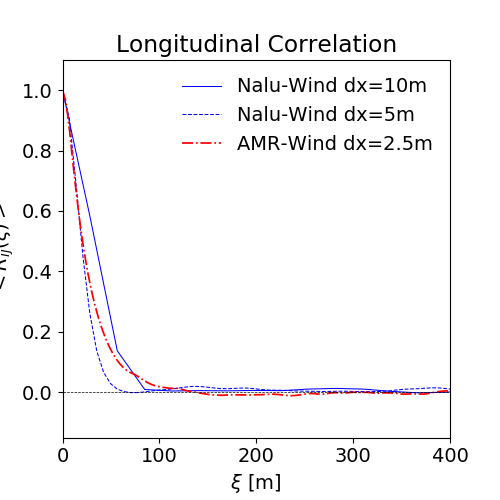
\includegraphics[width=3in]{figures/GridStudy_Rij_Longitudinal.png}
  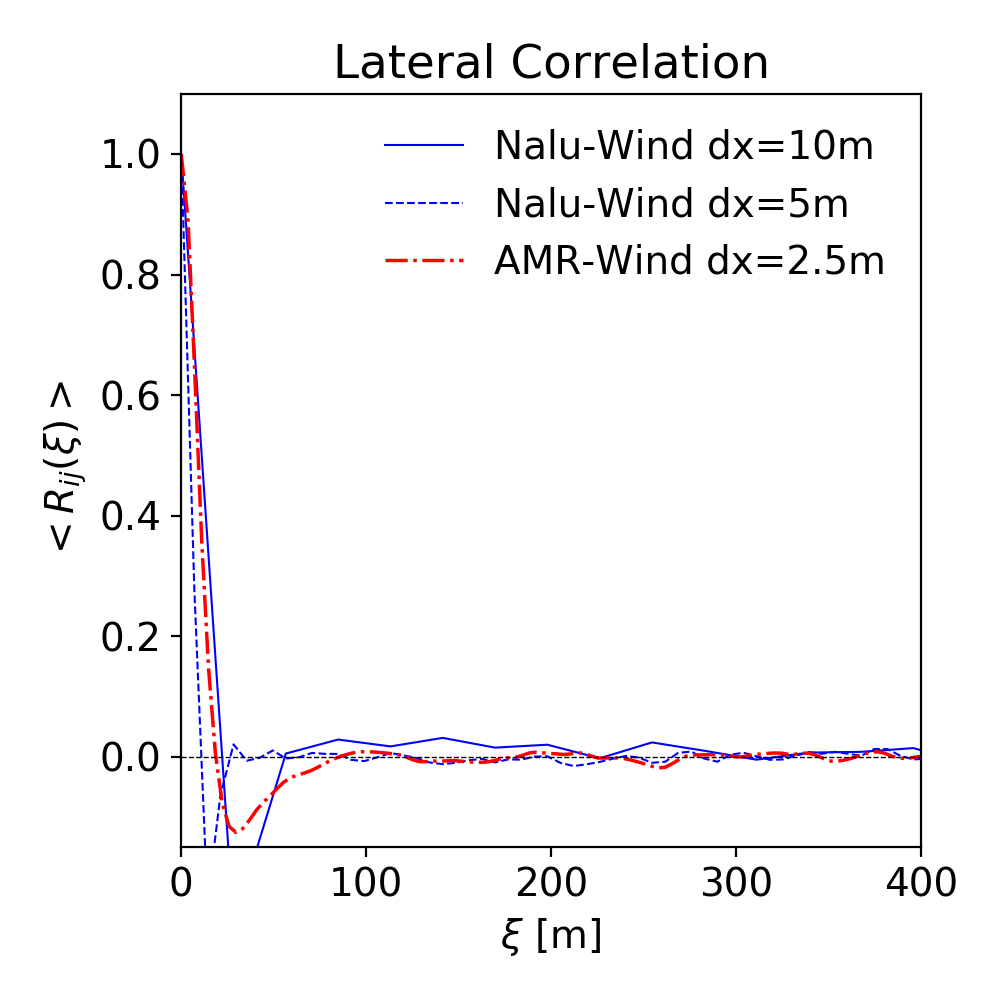
\includegraphics[width=3in]{figures/GridStudy_Rij_Lateral.png}
  \caption{Calculation of the averaged longitudinal and lateral
    $R_{ij}(\xi)$ coefficient at $z$=20m for LES of stable 5m/s case
    with different resolutions.}
\end{figure}
%%%%%%%%%%%%%%%%%%%%%%%%%%%%%%%%%%%%%%%%%%%%%%%%%%%%%%%%%%%%%%%%%%%%


The turbulent integral lengthscale can be calculated from $\langle
R_{ij}(\xi) \rangle$ via
\begin{equation}
  L = \int_0^\infty \langle R_{ij}(\xi) \rangle \: {\textrm d}\xi
\end{equation}

%%%%%%%%%%%%%%% GRID STUDY: INTEGRAL LENGTH %%%%%%%%%%%%%%%%%%%%%%%%%%%%%%%%%%%
\begin{table}
\caption{\label{tab:GridStudyLscale} The calculated turbulent integral
  lengthscale for each of the grid resolutions} \centering
\begin{tabular}{ccccc}
  \hline
  Case              & dx [m] & Longitudinal L [m] & Lateral L [m] \\
  \hline
  Nalu-wind coarse  &  10.0  & 36.433999          & 0.0        \\
  Nalu-wind medium  &   5.0  & 21.485711          & 4.519247   \\
  AMR-wind fine     &   2.5  & 27.689340          & 9.332672   \\
\hline
\end{tabular}
\end{table}

\subsection{Comparison of AMR-Wind vs Nalu-Wind}

\subsection{ABL Physics}

\subsubsection{ABL integrated quantities}
Describe integrated quantities

\subsubsection{Horizontally averaged profiles}

\subsubsection{Wind spectra and turbulence statistics}

The Kaimal model for spectra \cite{kaimal1973turbulence, cheynet2017spectral}
\begin{equation}
  \label{eq:kaimal}
  \frac{fS_i}{u_\tau^2} = \frac{a_i(fz/\bar{U})}{\left(1+b_i(fz/\bar{U})^{\alpha_i}\right)^{\beta_i}}
\end{equation}

%%%%%%%%%%%%%%% KAIMAL MODEL PARAMETERS %%%%%%%%%%%%%%%%%%%%%%%%%%%%%%%%%%%
\begin{table}
\caption{\label{tab:KaimalParameters} Parameters for Kaimal model}
\centering
\begin{tabular}{ccccc}
  \hline
  Velocity & $a_i$ & $b_i$ & $\alpha_i$  & $\beta_i$ \\
  \hline
  $u$      & 105.0 & 33.0  & 1           & 5/3  \\
  $v$      &  17.0 &  9.5  & 1           & 5/3  \\
  $w$      &   2.1 &  5.3  & 5/3         &   1  \\
\hline
\end{tabular}
\end{table}

\subsubsection{Comparison with neutral and unstable conditions}


%%%%%%%%%%% All stability correlation figure %%%%%%%%%%%%%%%%%%%%
% created in Postprocessing/ABLLength/CompareAll_ABL_Lengthscales.ipynb 
\begin{figure}[hbt!]
  \label{fig:AllStabilityRij}
  \centering
  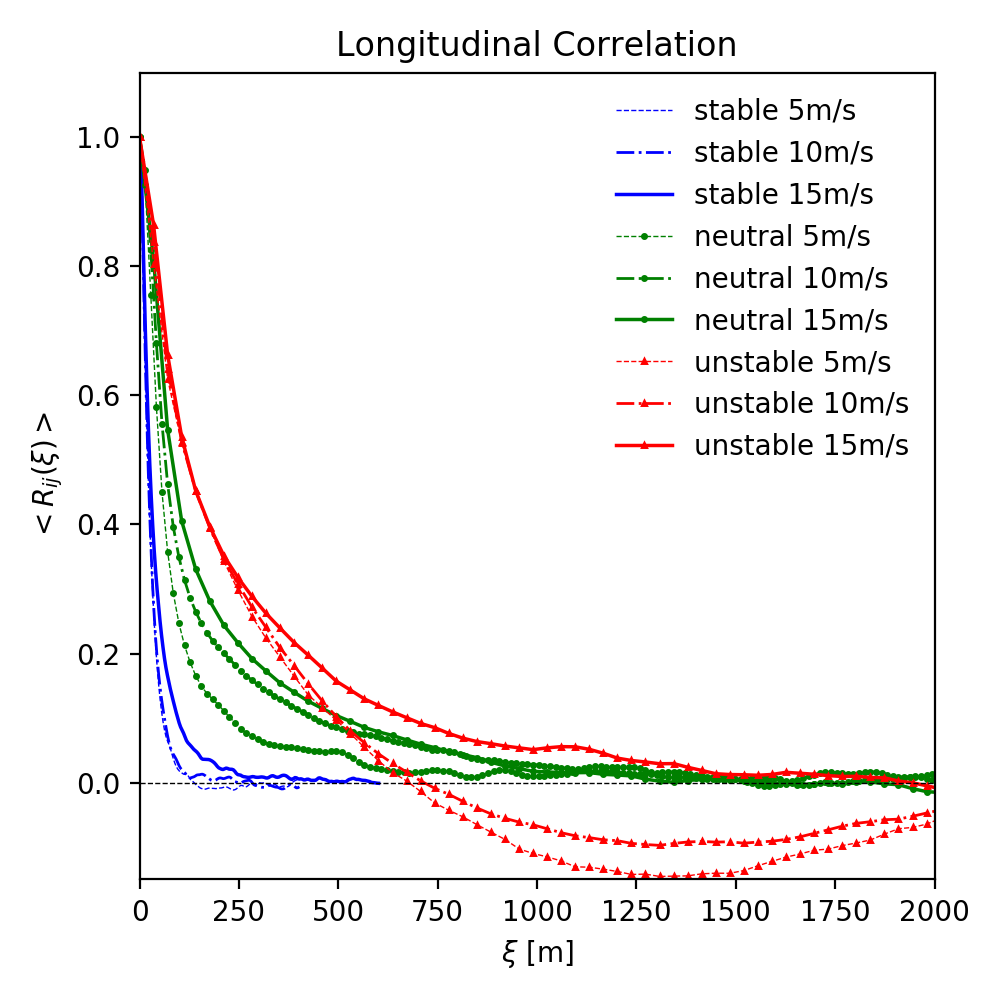
\includegraphics[width=3in]{figures/AllStability_Rij_Longitudinal.png}
  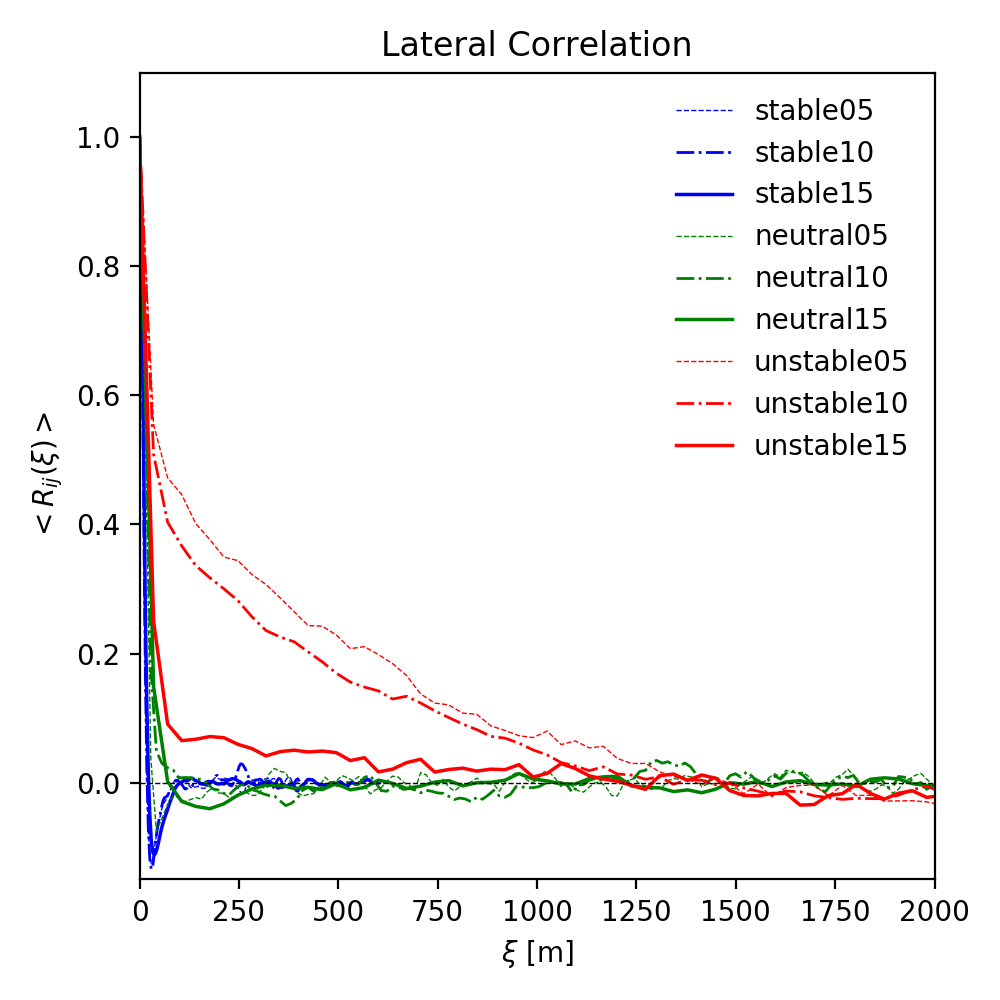
\includegraphics[width=3in]{figures/AllStability_Rij_Lateral.png}
  \caption{Calculation of the averaged longitudinal and lateral
    $R_{ij}(\xi)$ coefficient at $z$=20m for all ABL stability cases.}
\end{figure}
%%%%%%%%%%%%%%%%%%%%%%%%%%%%%%%%%%%%%%%%%%%%%%%%%%%%%%%%%%%%%%%%%%%%
